\documentclass[11pt]{standalone}
\usepackage[usenames]{color} %used for font color
\usepackage{amssymb} %maths
\usepackage{amsmath} %maths

\usepackage[no-math]{fontspec}
\usepackage{unicode-math}
\setmainfont{Lato}
\setmathfont{Stix Two Math}

\usepackage{pgf,xcolor}
\definecolor{itwm_blue_04}{HTML}{005A94}
\definecolor{itwm_red}{HTML}{C00000}
\definecolor{itwm_yellow}{HTML}{FFEC7F}

\usepackage{tikz}
\usetikzlibrary{shapes.misc, shadows, decorations, arrows}
\usetikzlibrary{backgrounds}
\usetikzlibrary{calc}
\usepackage{pgfplots}
\pgfplotsset{compat=newest}
\usepgfplotslibrary{fillbetween}
\usepackage{tikzpagenodes}

\begin{document}
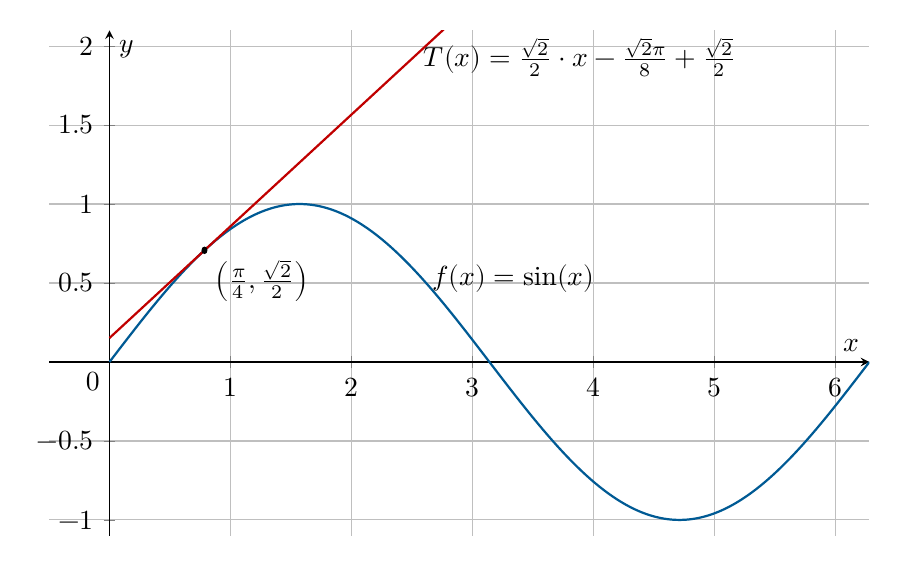
\begin{tikzpicture}
\begin{axis}[
    domain=0:2*pi,
    axis lines = center,
    xlabel = {$x$},
    ylabel = {$y$},
    height=8cm, width=12cm, 
    xmin=-0.5, xmax=2*pi, ymin=-1.1, ymax=2.1, 
    xtick={-1, 0,...,6},
    ytick={-1, -0.5, 0,...,2},
    grid = both
]
\addplot[draw=itwm_blue_04, samples=300, thick, name path=f]{sin(deg(x))} node [pos=0.4, right] {$f(x)=\sin(x)$};
\addplot[draw=itwm_red, samples=300, thick, name path=T]{0.707*x - 0.707*3.14159/4 + 0.707} node [pos=0.4, right] {$T(x) = \frac{\sqrt{2}}{2} \cdot x - \frac{\sqrt{2}\pi}{8} + \frac{\sqrt{2}}{2}$};
%\draw[domain=0:3,smooth,variable=\x,itwm_red, thick] plot ({\x},{0.707*\x - 0.707*3.14159/4 + 0.707}) node[below right] {$T(x)$};
    \filldraw[black] ({pi/4},{sin(deg(pi/4))}) circle (0.02) 
        node[below right] {$\left(\frac{\pi}{4}, \frac{\sqrt{2}}{2}\right)$};
    \node[below left] at (0,0) {0};
\end{axis}
\end{tikzpicture}
\end{document}

